\documentclass[ignorenonframetext,]{beamer}
\usetheme{Marburg}
\usepackage{amssymb,amsmath}
\usepackage{ifxetex,ifluatex}
\usepackage{fixltx2e} % provides \textsubscript
\usepackage{lmodern}
\ifxetex
  \usepackage{fontspec,xltxtra,xunicode}
  \defaultfontfeatures{Mapping=tex-text,Scale=MatchLowercase}
  \newcommand{\euro}{€}
\else
  \ifluatex
    \usepackage{fontspec}
    \defaultfontfeatures{Mapping=tex-text,Scale=MatchLowercase}
    \newcommand{\euro}{€}
  \else
    \usepackage[T1]{fontenc}
    \usepackage[utf8]{inputenc}
      \fi
\fi
\IfFileExists{upquote.sty}{\usepackage{upquote}}{}
% use microtype if available
\IfFileExists{microtype.sty}{\usepackage{microtype}}{}
\usepackage{longtable,booktabs}
\usepackage{caption}
% These lines are needed to make table captions work with longtable:
\makeatletter
\def\fnum@table{\tablename~\thetable}
\makeatother
\usepackage{letltxmacro}
\makeatletter
\def\maxwidth{\ifdim\Gin@nat@width>\linewidth\linewidth\else\Gin@nat@width\fi}
\def\maxheight{\ifdim\Gin@nat@height>\textheight0.8\textheight\else\Gin@nat@height\fi}
\makeatother
\AtBeginDocument{
  \LetLtxMacro\Oldincludegraphics\includegraphics
  \renewcommand{\includegraphics}[2][]{%
    \Oldincludegraphics[#1,width=\maxwidth,height=\maxheight,keepaspectratio]{#2}}
}

% Comment these out if you don't want a slide with just the
% part/section/subsection/subsubsection title:
\AtBeginPart{
  \let\insertpartnumber\relax
  \let\partname\relax
  \frame{\partpage}
}
\AtBeginSection{
  \let\insertsectionnumber\relax
  \let\sectionname\relax
  \frame{\sectionpage}
}
\AtBeginSubsection{
  \let\insertsubsectionnumber\relax
  \let\subsectionname\relax
  \frame{\subsectionpage}
}

\setlength{\parindent}{0pt}
\setlength{\parskip}{6pt plus 2pt minus 1pt}
\setlength{\emergencystretch}{3em}  % prevent overfull lines
\setcounter{secnumdepth}{0}

\title{GAMUT Update}
\author{GAMUT Database}
\date{Sunday, Sept 7, 2014}

\begin{document}
\frame{\titlepage}

\section{Participation}\label{participation}

\begin{frame}{GAMUT Overview}

\begin{block}{62 Total programs enrolled}

\begin{itemize}
\item
  26 reporting data\\
\item
  36 not reporting data
\item
  8 reporting all of 2014 YTD
\end{itemize}

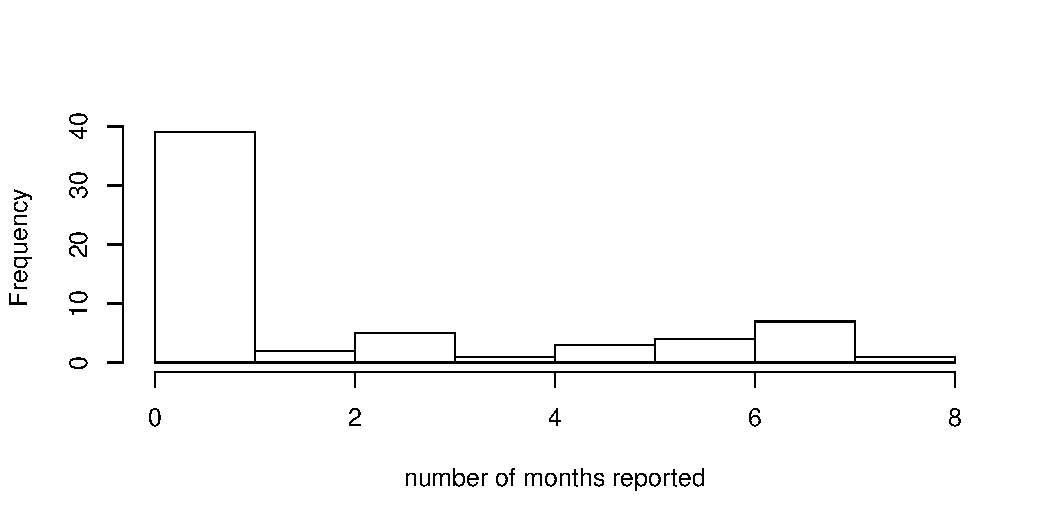
\includegraphics{figures/hist_reporting.pdf}

\end{block}

\end{frame}

\begin{frame}{Patients}

\begin{block}{14347 Total Patients}

\begin{itemize}
\itemsep1pt\parskip0pt\parsep0pt
\item
  3780 Neonatal\\
\item
  8151 Pediatric\\
\item
  2409 Adult
\end{itemize}

Data as of : Sun Sep 07 11:55:04 2014

\end{block}

\end{frame}

\section{Advanced Airway Management}\label{advanced-airway-management}

\begin{frame}{Mechanical Ventilation}

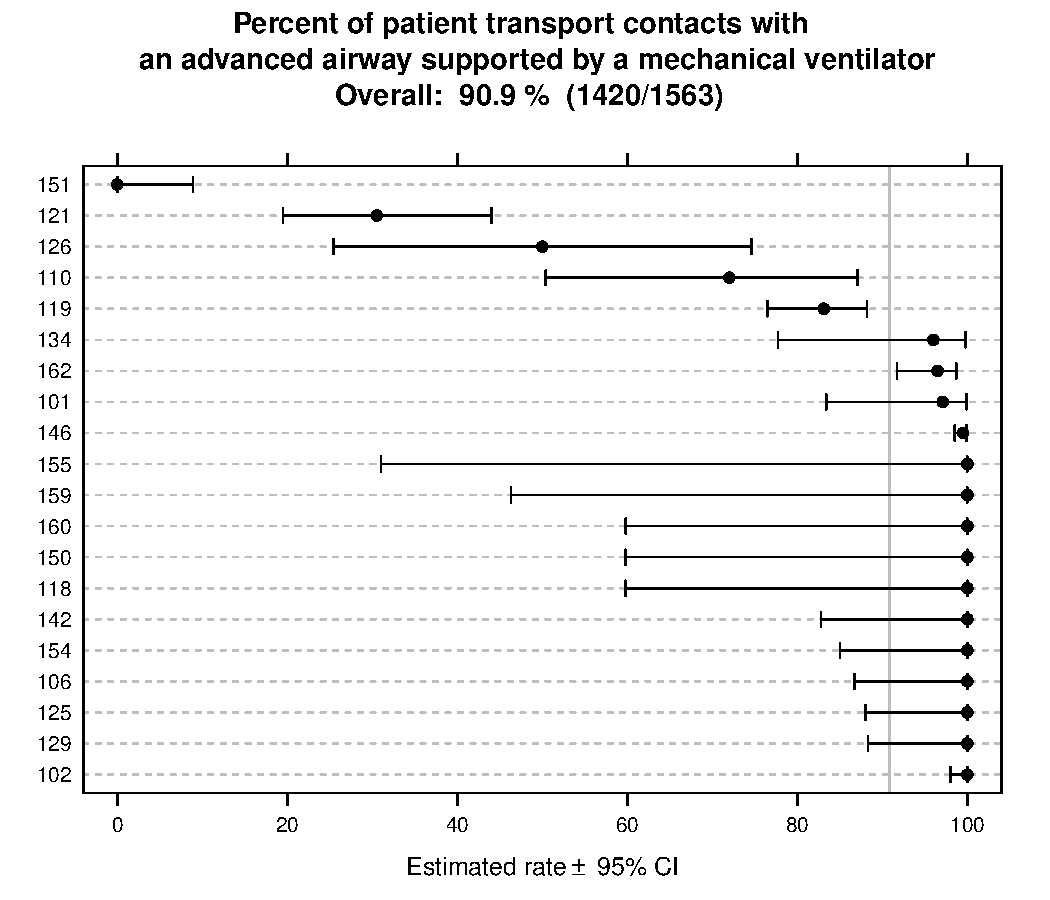
\includegraphics{figures/vent_adv_airway.pdf}

\end{frame}

\begin{frame}{Waveform Capnography}

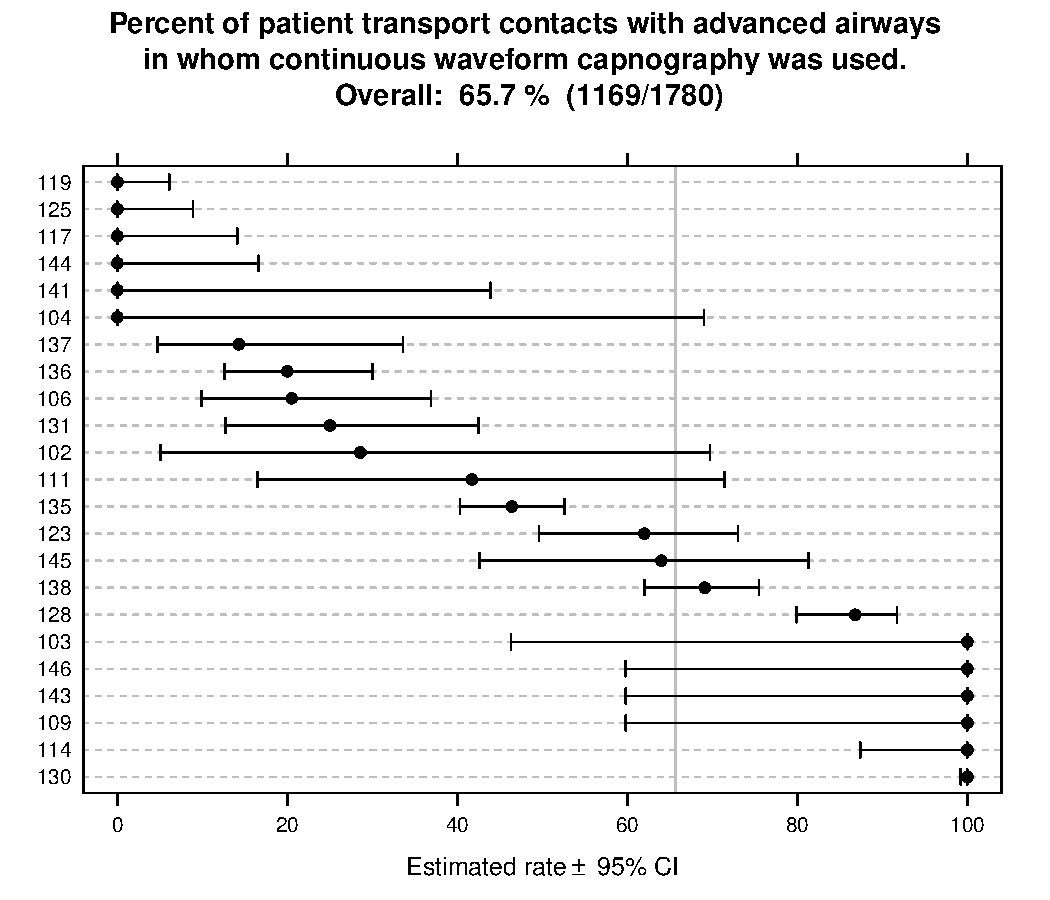
\includegraphics{figures/waveform_capno.pdf}

\end{frame}

\begin{frame}{Confirmed tracheal tube placement}

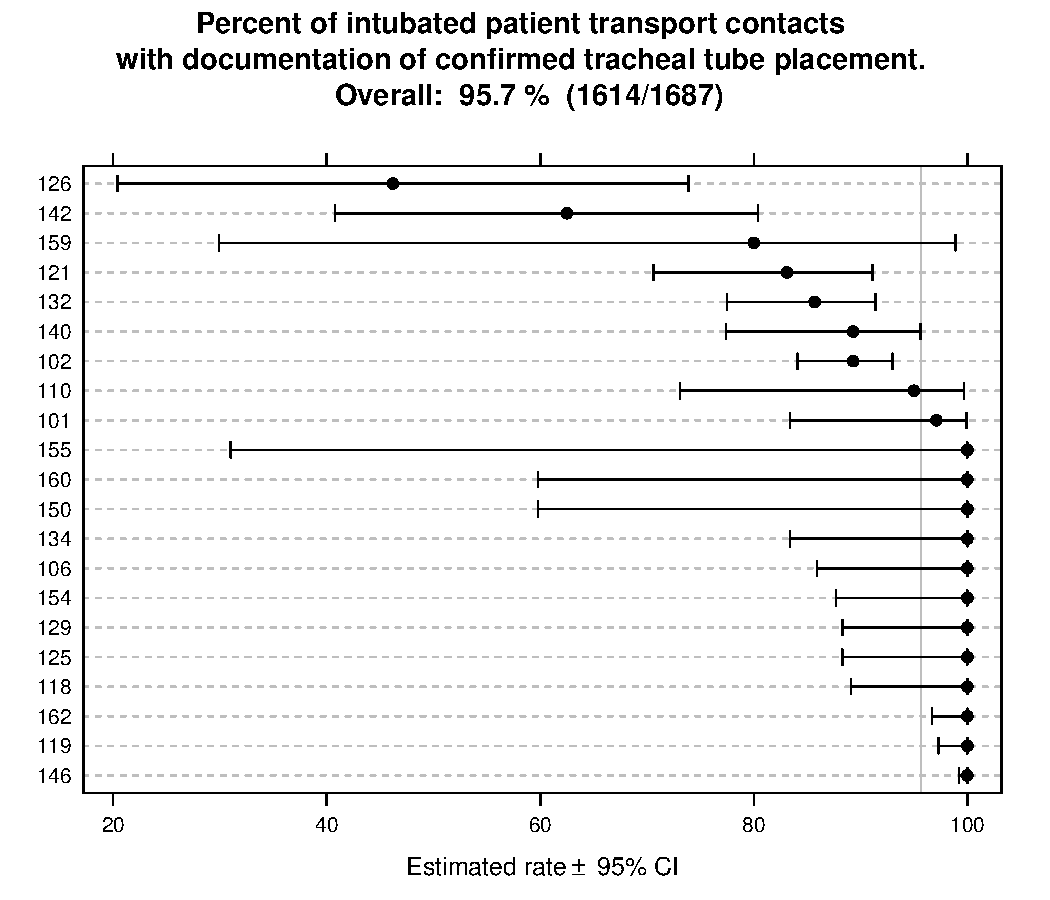
\includegraphics{figures/confirmed_tt.pdf}

\end{frame}

\section{Intubation}\label{intubation}

\begin{frame}{Neonatal - First Attempt Success}

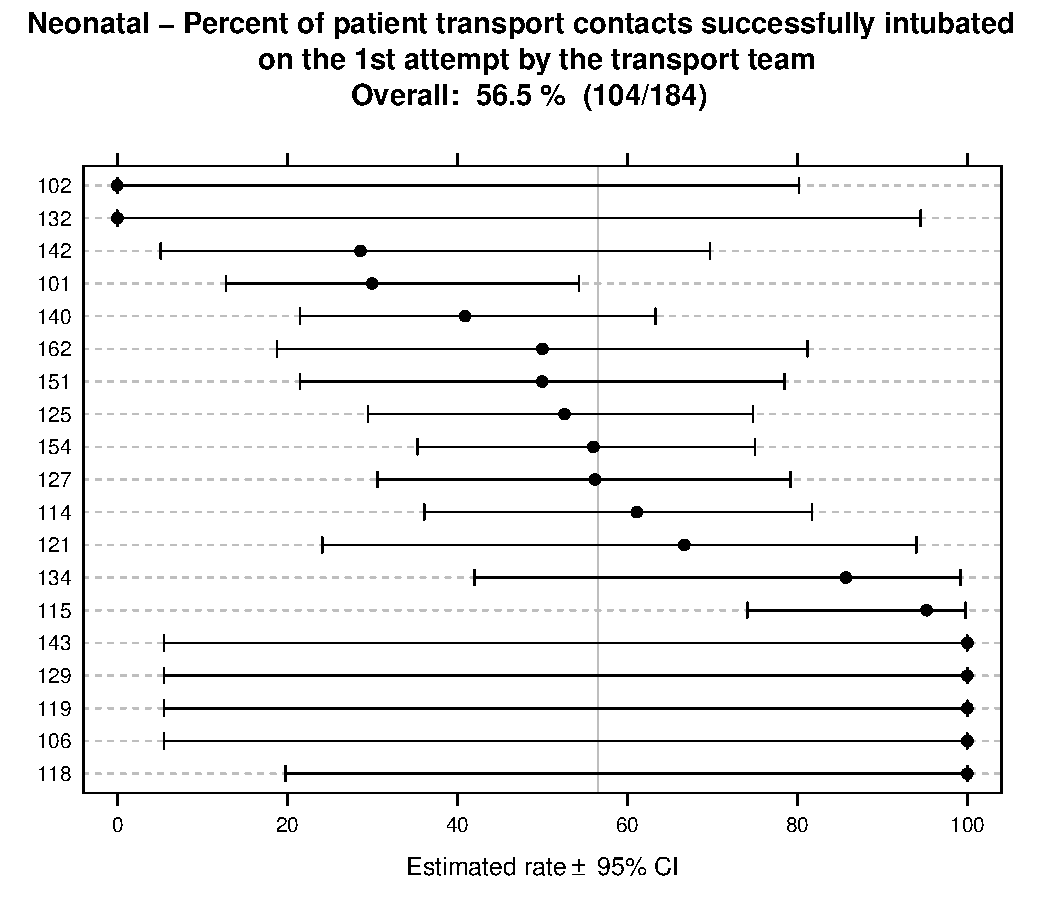
\includegraphics{figures/first_attempt_success_neo.pdf}

\end{frame}

\begin{frame}{Neonatal - DASH-1A}

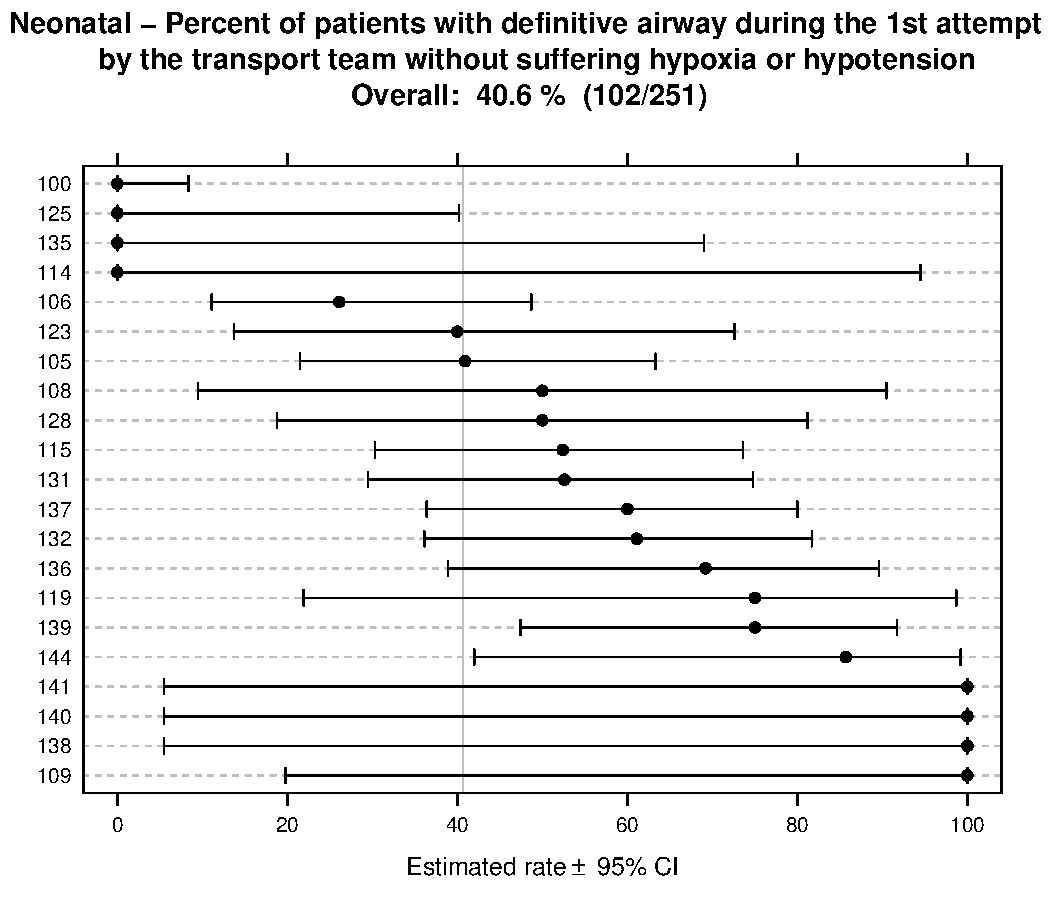
\includegraphics{figures/DASH1A_neo.pdf}

\end{frame}

\begin{frame}{Pediatric - First Attempt Success}

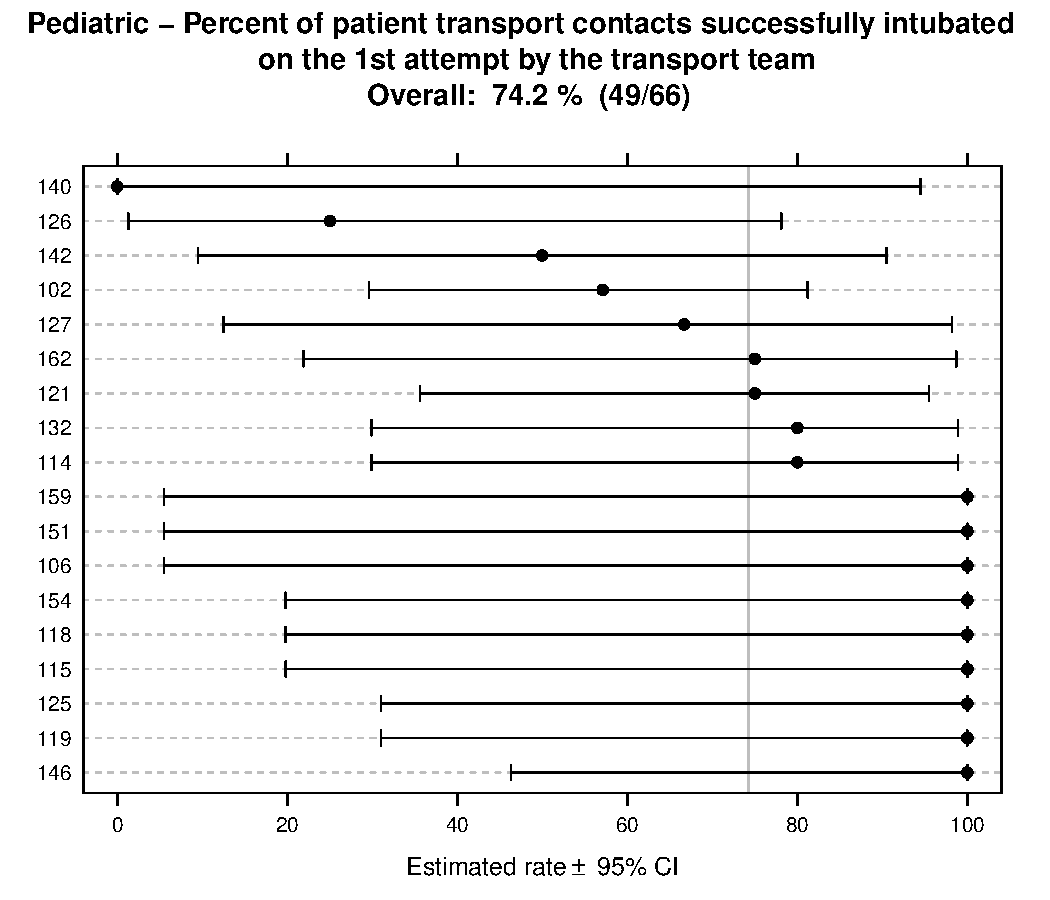
\includegraphics{figures/first_attempt_success_ped.pdf}

\end{frame}

\begin{frame}{Pediatric - DASH-1A}

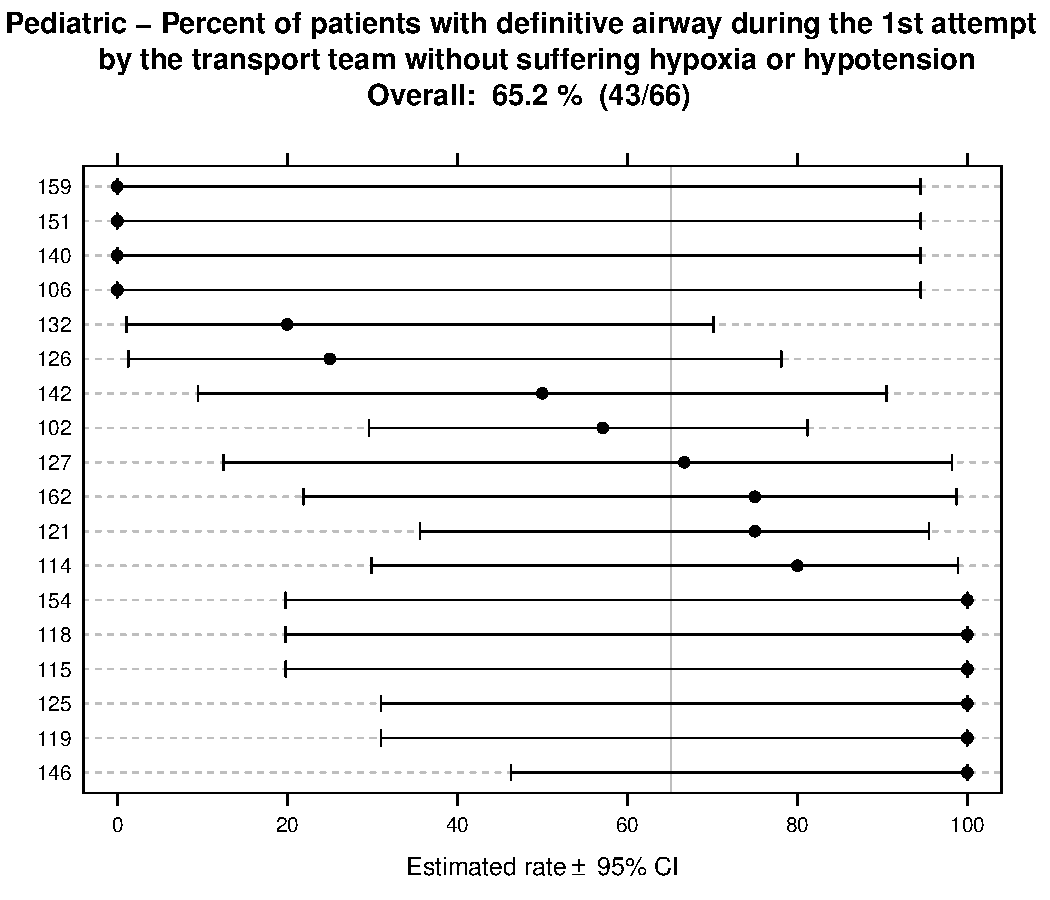
\includegraphics{figures/DASH1A_ped.pdf}

\end{frame}

\begin{frame}{Adult - First Attempt Success}

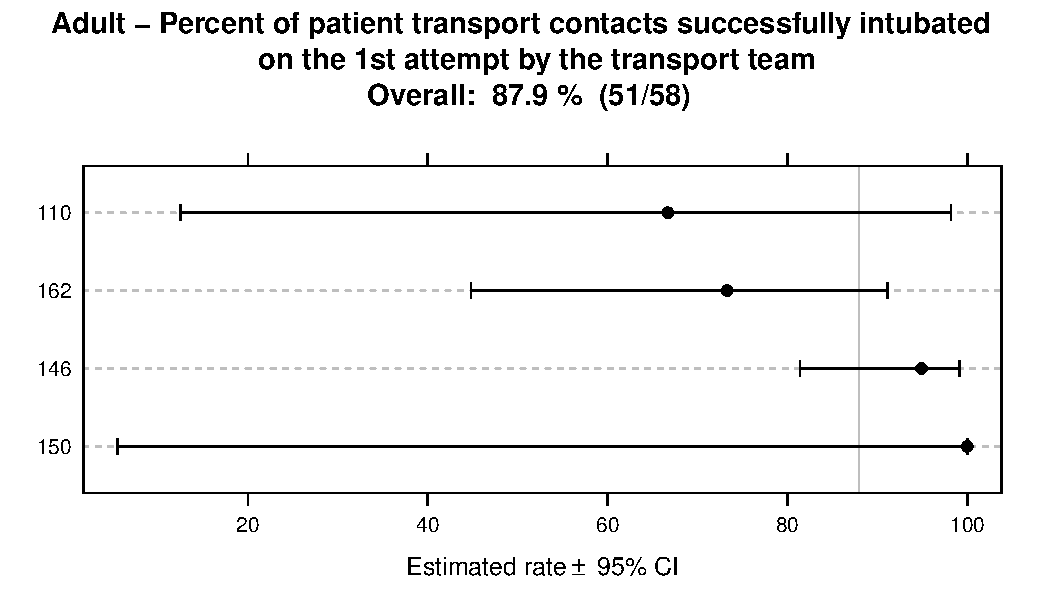
\includegraphics{figures/first_attempt_success_adult.pdf}

\end{frame}

\begin{frame}{Adult DASH-1A}

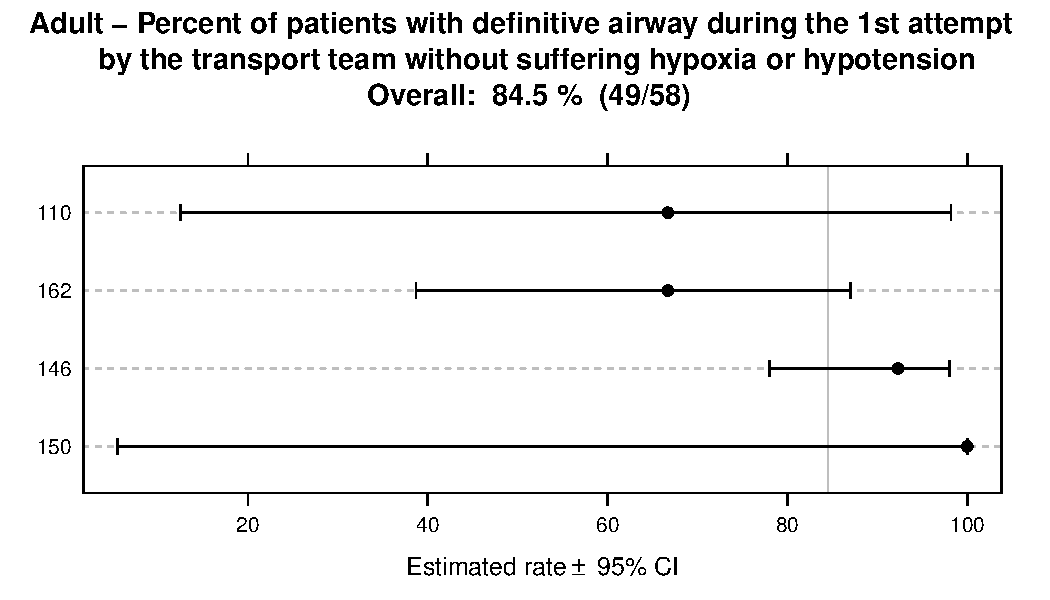
\includegraphics{figures/DASH1A_adult.pdf}

\end{frame}

\begin{frame}{RSI protocol compliance}

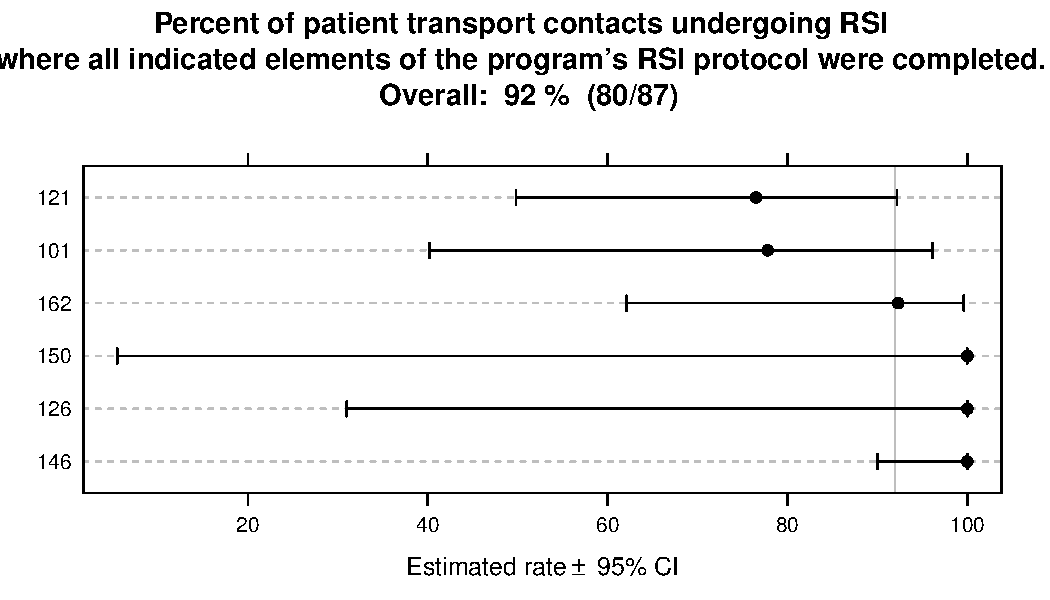
\includegraphics{figures/RSI_compliance.pdf}

\end{frame}

\section{General Metrics}\label{general-metrics}

\begin{frame}{Reliable pain assessments}

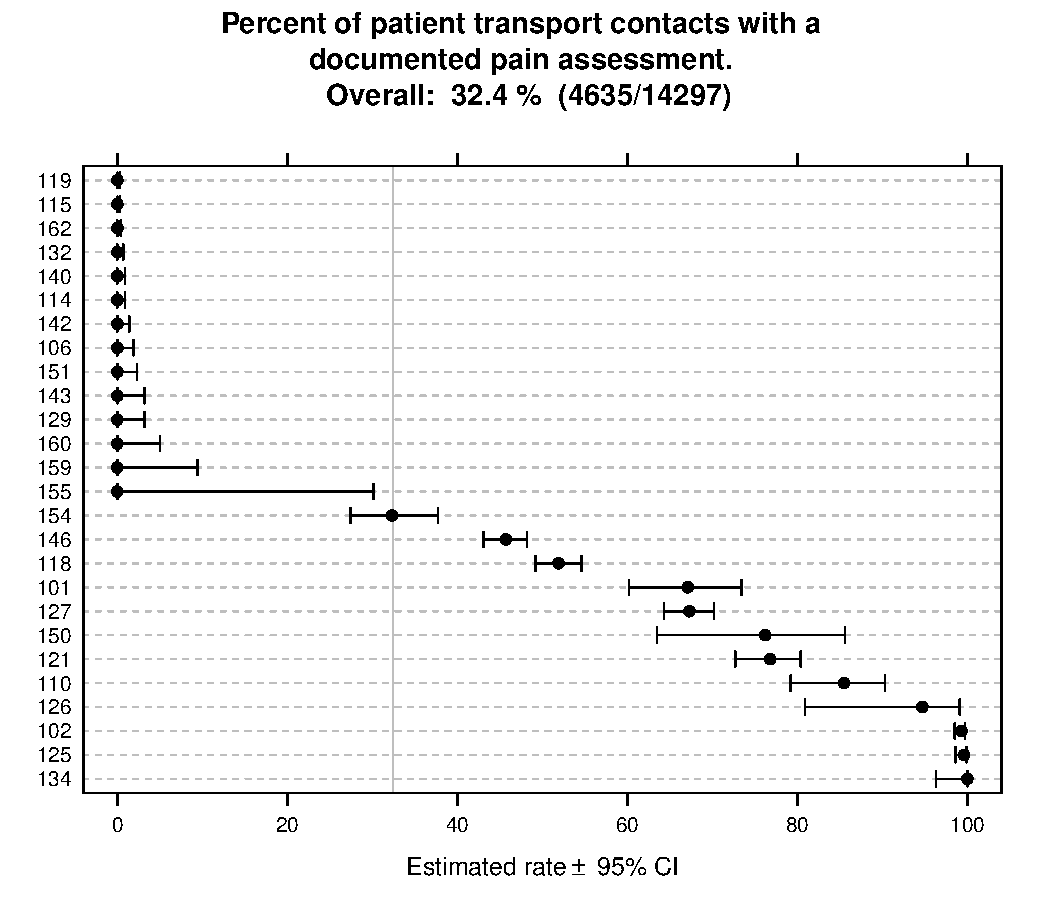
\includegraphics{figures/pain_assessment.pdf}

\end{frame}

\begin{frame}{Incidence of hypoxia during transport}

\begin{block}{NUMERATOR:}

Number of patient transport contacts during which the documented pulse
oximetry reading drops below 90\%.

Multiple incidents with one patient are considered as one incident. If
the pulse oximetry reading is chronically low or is below 90\% when
contact is made, the patient is not included except for those patients
where the saturation has been corrected to greater than 90\% and falls
again.

\end{block}

\begin{block}{DENOMINATOR:}

Number of patient transport contacts during the calendar month
(excluding those with chronic oxygen saturations lower than 90\% or
oxygen saturations lower than 90\% that persist throughout the entire
transport).

\end{block}

\end{frame}

\begin{frame}{Incidence of hypoxia during transport}

\begin{longtable}[c]{@{}rrr@{}}
\toprule\addlinespace
group & num & den
\\\addlinespace
\midrule\endhead
101 & 11 & 205
\\\addlinespace
102 & 2 & 894
\\\addlinespace
106 & 0 & 0
\\\addlinespace
110 & 9 & 168
\\\addlinespace
114 & 0 & 0
\\\addlinespace
115 & 0 & 0
\\\addlinespace
118 & 0 & 0
\\\addlinespace
\bottomrule
\end{longtable}

\end{frame}

\begin{frame}{Incidence of hypoxia during transport}

\begin{longtable}[c]{@{}rrr@{}}
\toprule\addlinespace
group & num & den
\\\addlinespace
\midrule\endhead
119 & 2 & 0
\\\addlinespace
121 & 0 & 0
\\\addlinespace
125 & 0 & 0
\\\addlinespace
126 & 4 & 0
\\\addlinespace
127 & 0 & 0
\\\addlinespace
129 & 0 & 0
\\\addlinespace
132 & 0 & 0
\\\addlinespace
\bottomrule
\end{longtable}

\end{frame}

\begin{frame}{Incidence of hypoxia during transport}

\begin{longtable}[c]{@{}rrr@{}}
\toprule\addlinespace
group & num & den
\\\addlinespace
\midrule\endhead
134 & 0 & 127
\\\addlinespace
140 & 0 & 0
\\\addlinespace
142 & 0 & 0
\\\addlinespace
143 & 0 & 0
\\\addlinespace
146 & 3 & 4
\\\addlinespace
150 & 1 & 63
\\\addlinespace
\bottomrule
\end{longtable}

\end{frame}

\begin{frame}{HEMS Over-triage}

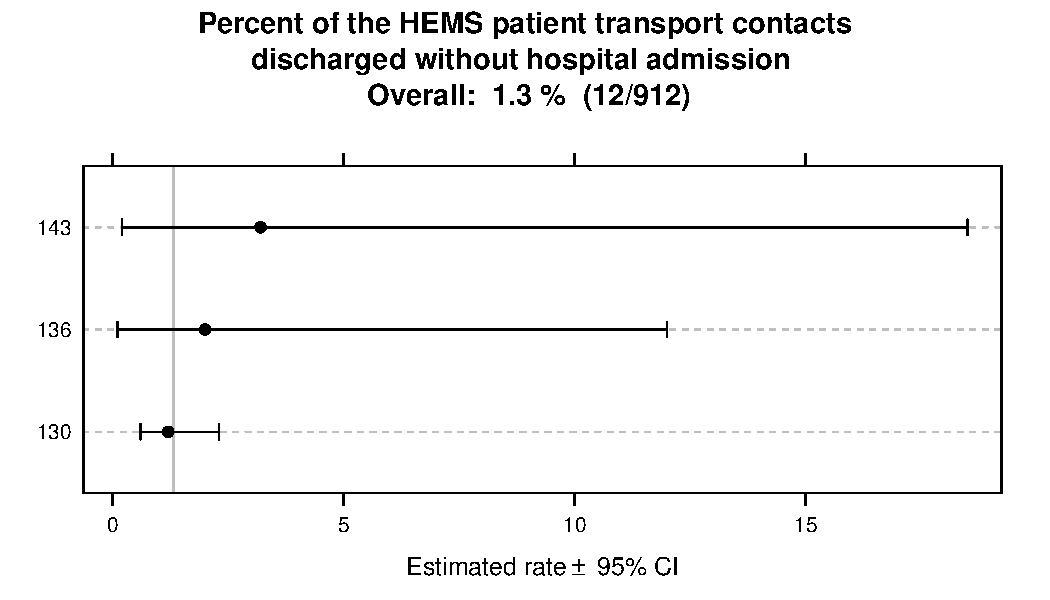
\includegraphics{figures/hems_over_triage.pdf}

\end{frame}

\section{Focused Populations}\label{focused-populations}

\begin{frame}{Neonatal Hypothermia on Arrival}

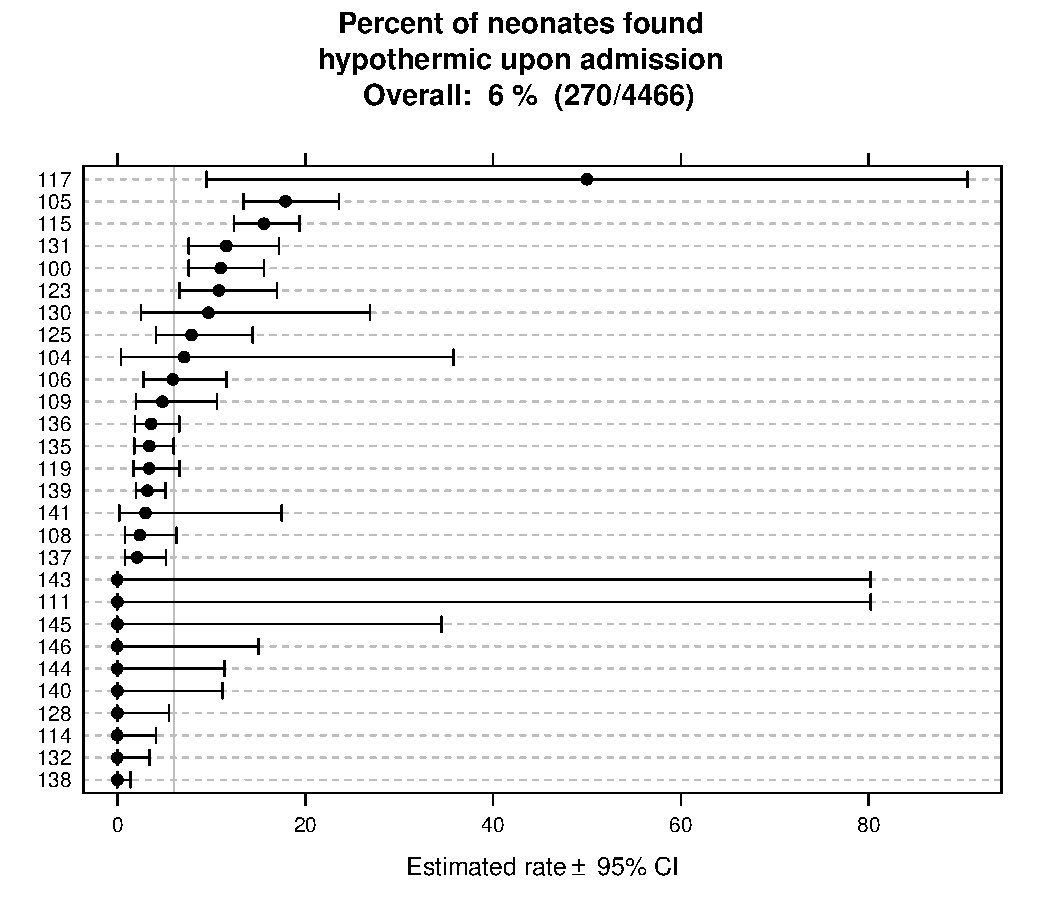
\includegraphics{figures/neonatal_hypothermia.pdf}

\end{frame}

\begin{frame}{STEMI Bedside}

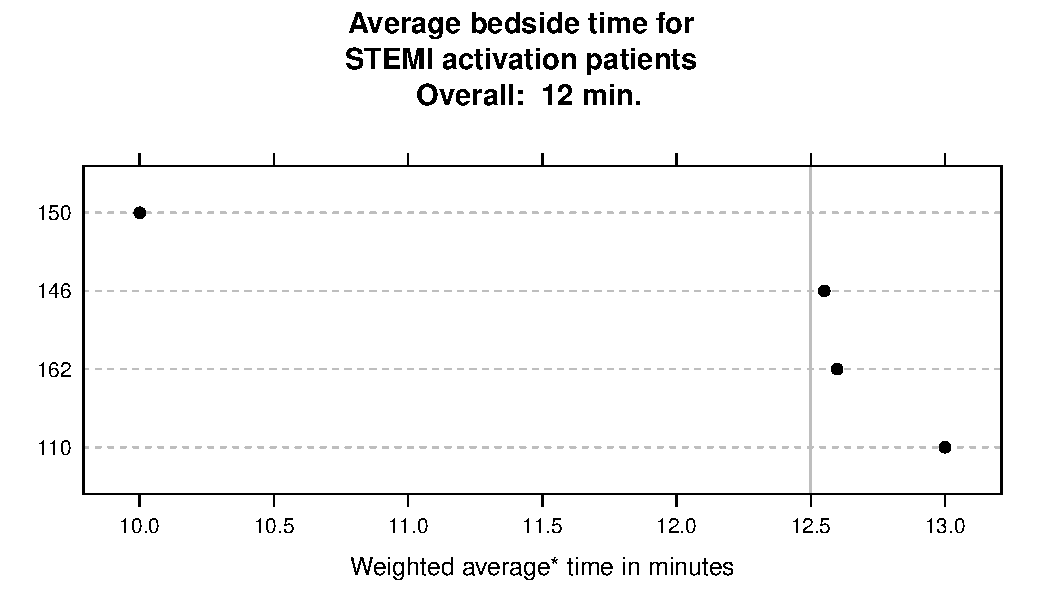
\includegraphics{figures/bedside_stemi.pdf}

\end{frame}

\begin{frame}{STEMI Scene}

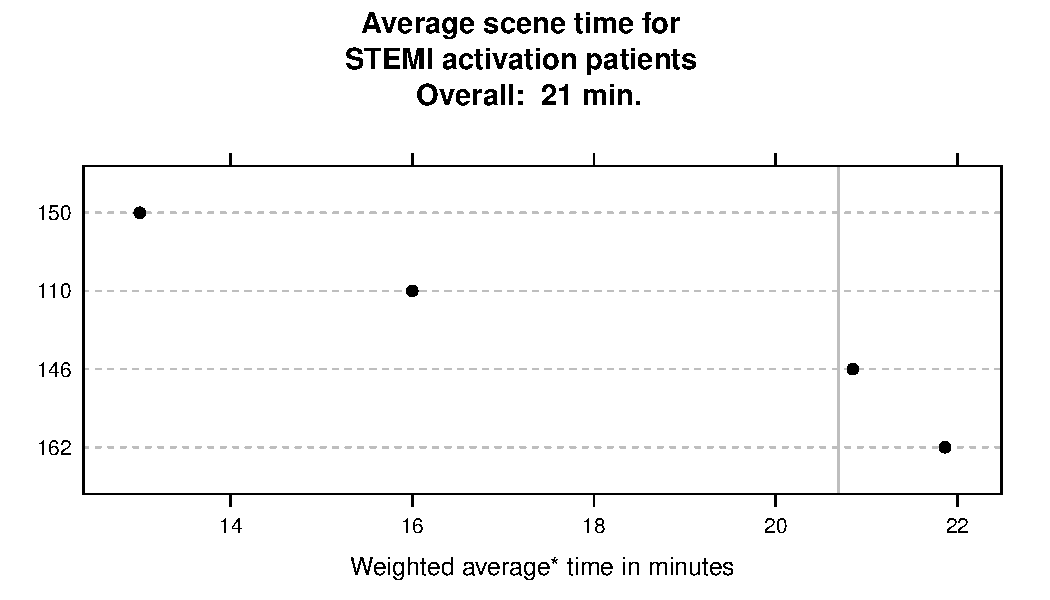
\includegraphics{figures/scene_stemi.pdf}

\end{frame}

\begin{frame}{ECG interpretation for STEMI patients}

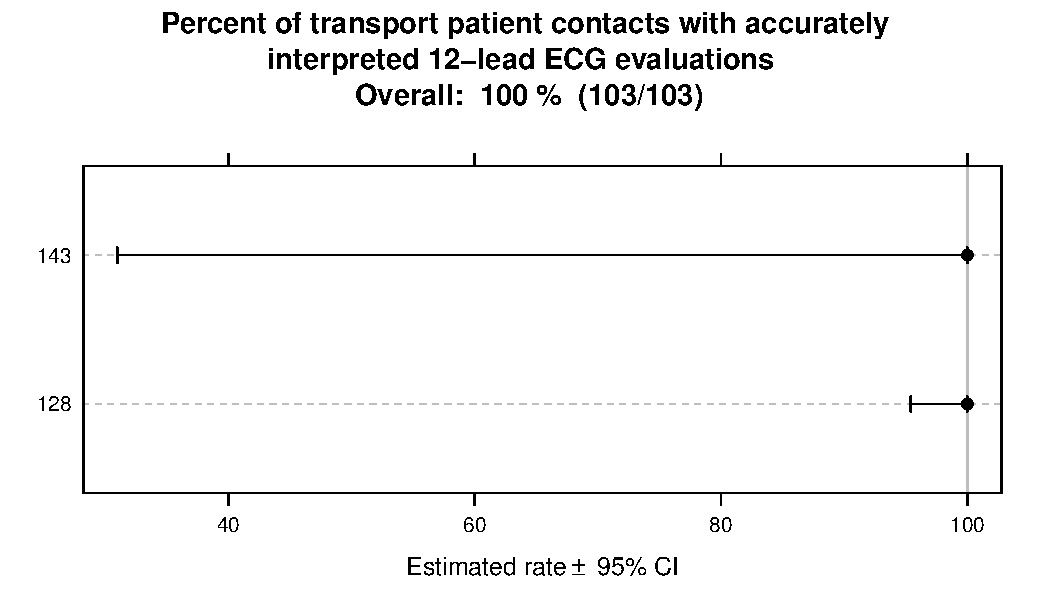
\includegraphics{figures/ecg_stemi.pdf}

\end{frame}

\begin{frame}{Blood glucose check for altered mental status}

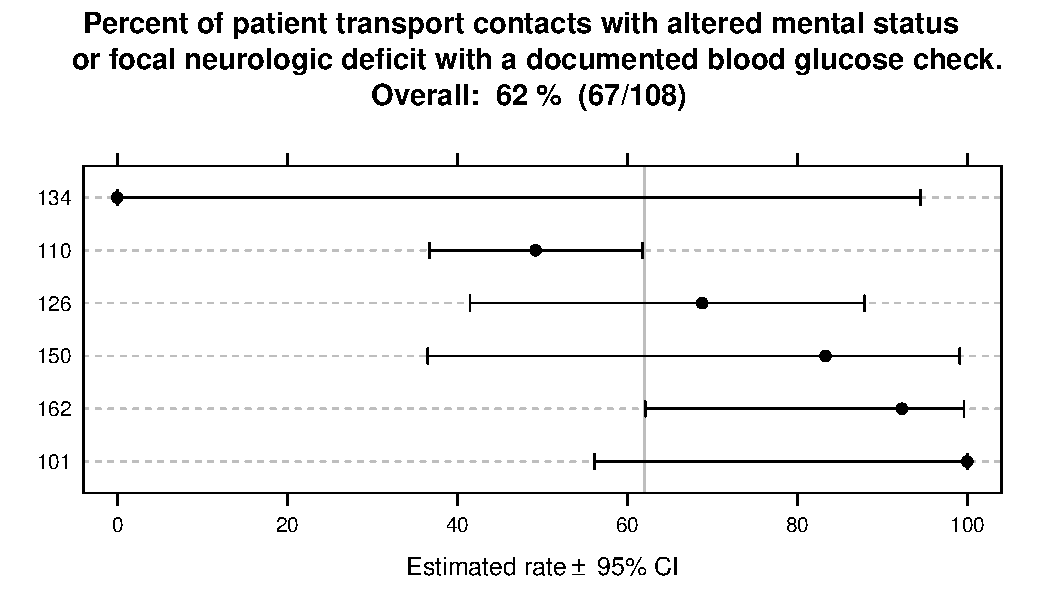
\includegraphics{figures/bg_check.pdf}

\end{frame}

\begin{frame}{Management of hypertension in hemorrhagic stroke}

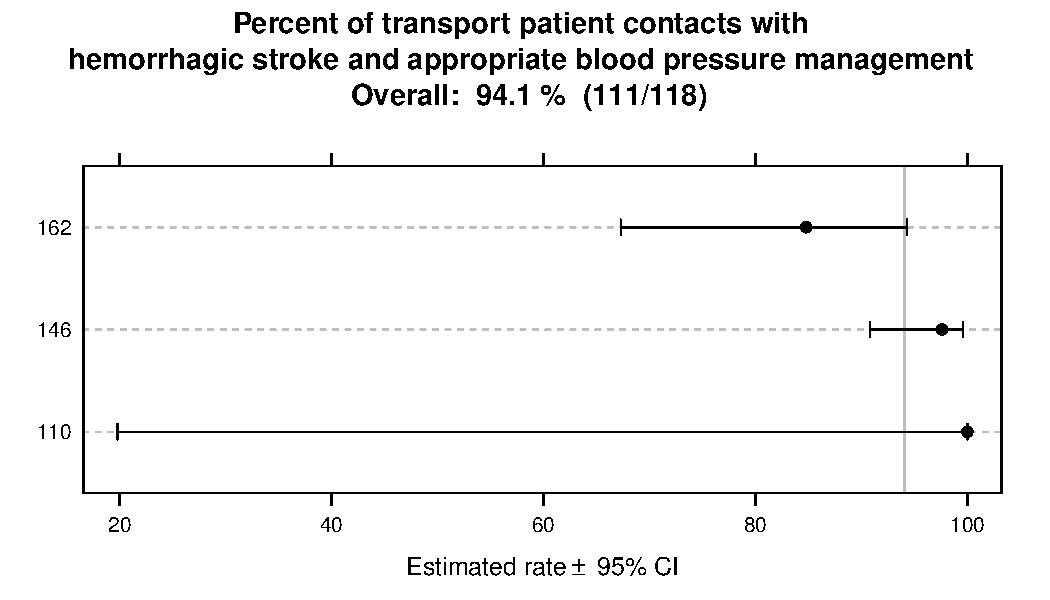
\includegraphics{figures/htn_hem_stroke.pdf}

\end{frame}

\begin{frame}{Appropriate management of hemorrhagic shock}

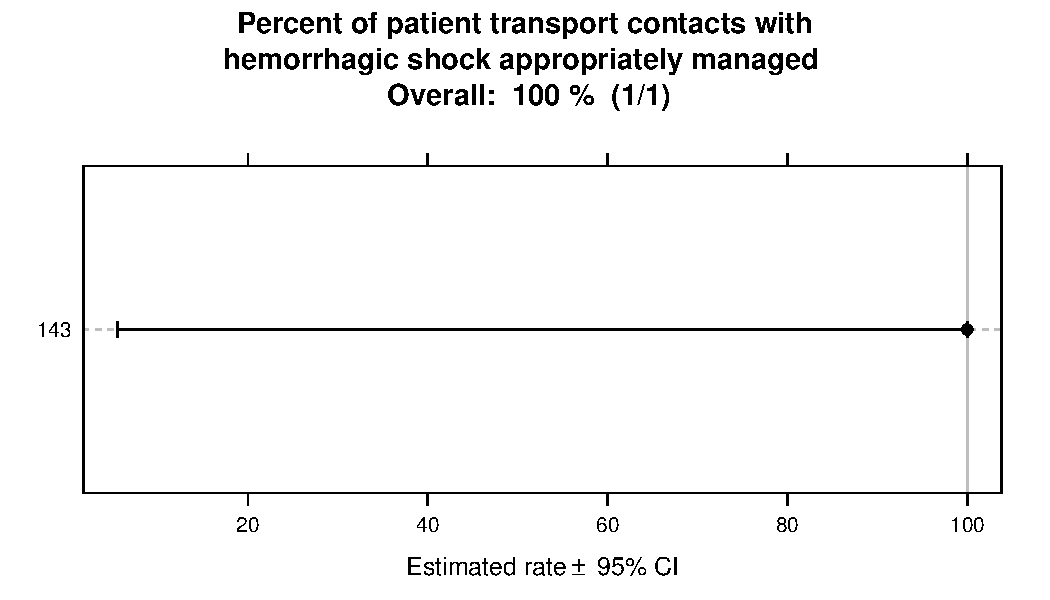
\includegraphics{figures/hem_shock_managed.pdf}

\end{frame}

\begin{frame}{Appropriate management of blood pressure for aortic
emergencies}

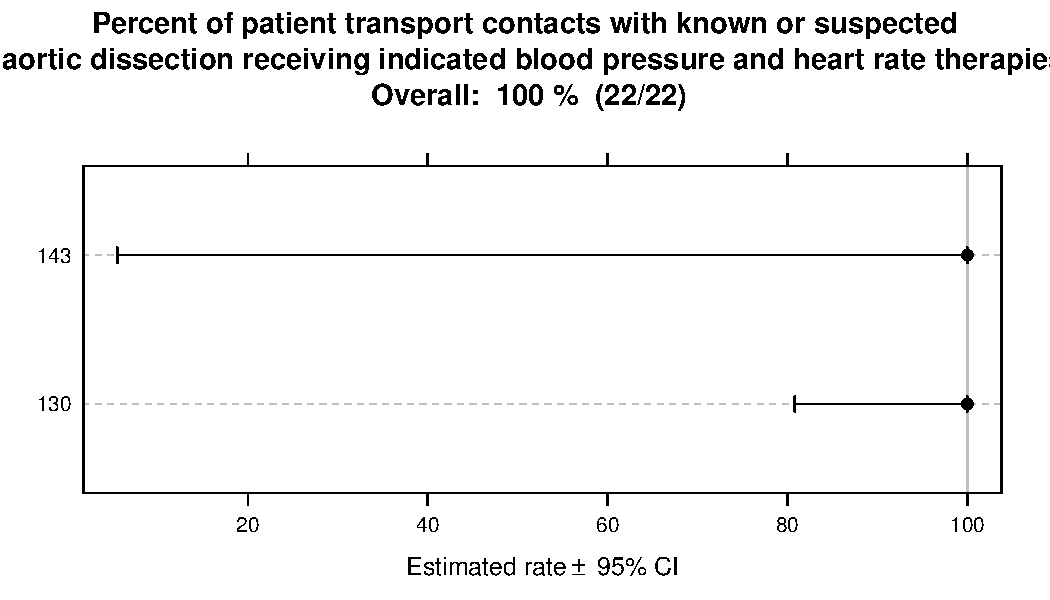
\includegraphics{figures/bp_aortic.pdf}

\end{frame}

\section{Rare Events}\label{rare-events}

\begin{frame}{Medical equipment failure}

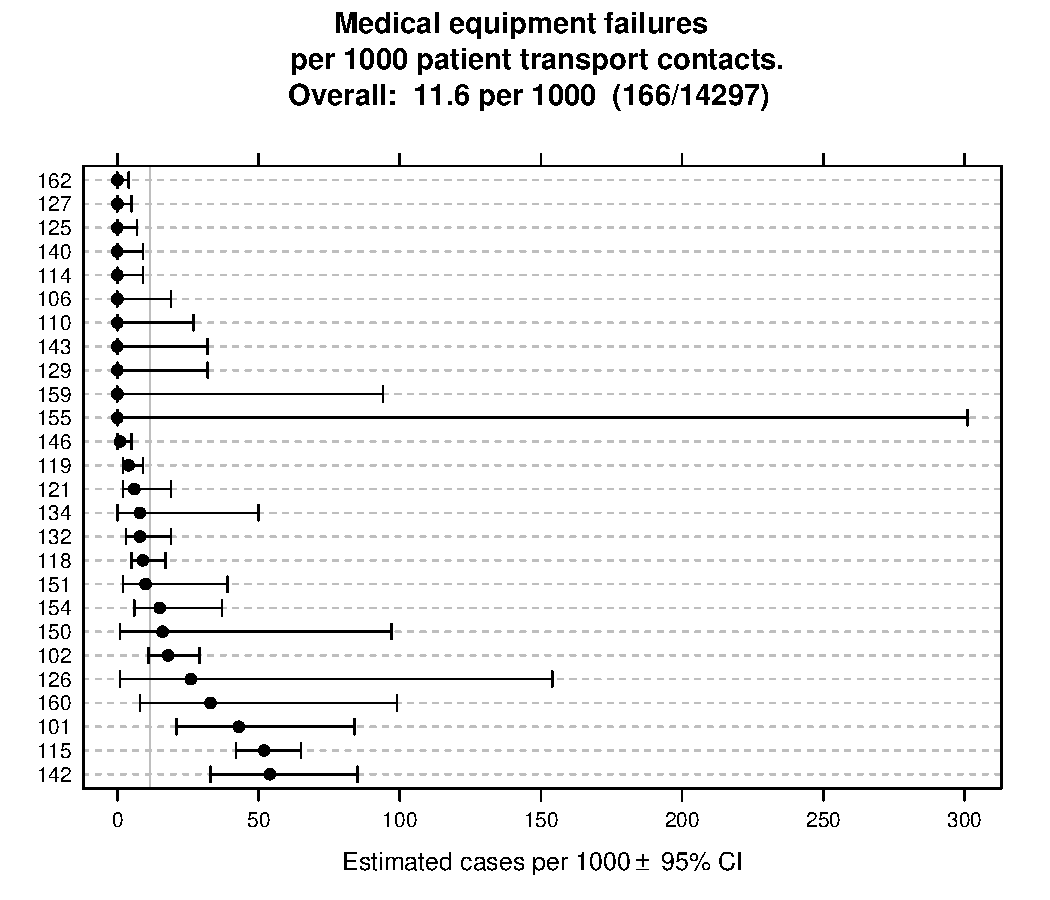
\includegraphics{figures/med_equip_failure.pdf}

\end{frame}

\begin{frame}{Adverse drug event during transport}

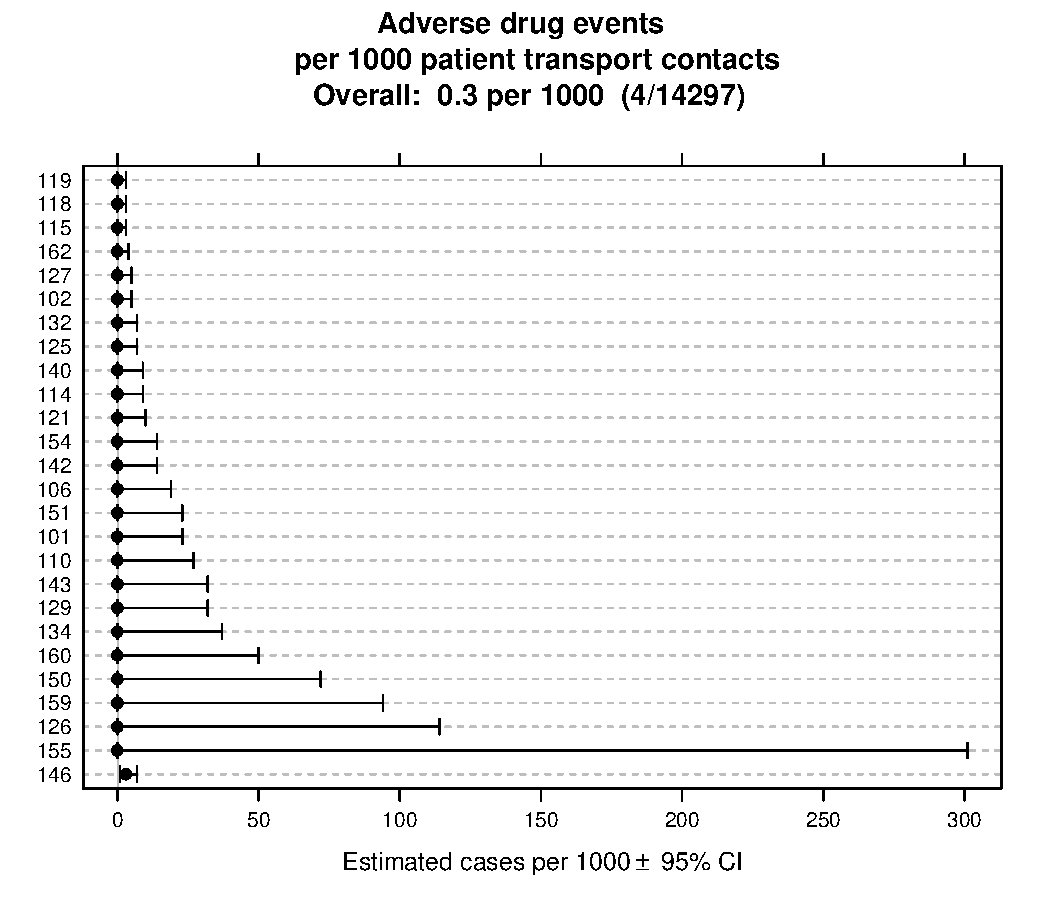
\includegraphics{figures/ade.pdf}

\end{frame}

\begin{frame}{Patient near-miss events}

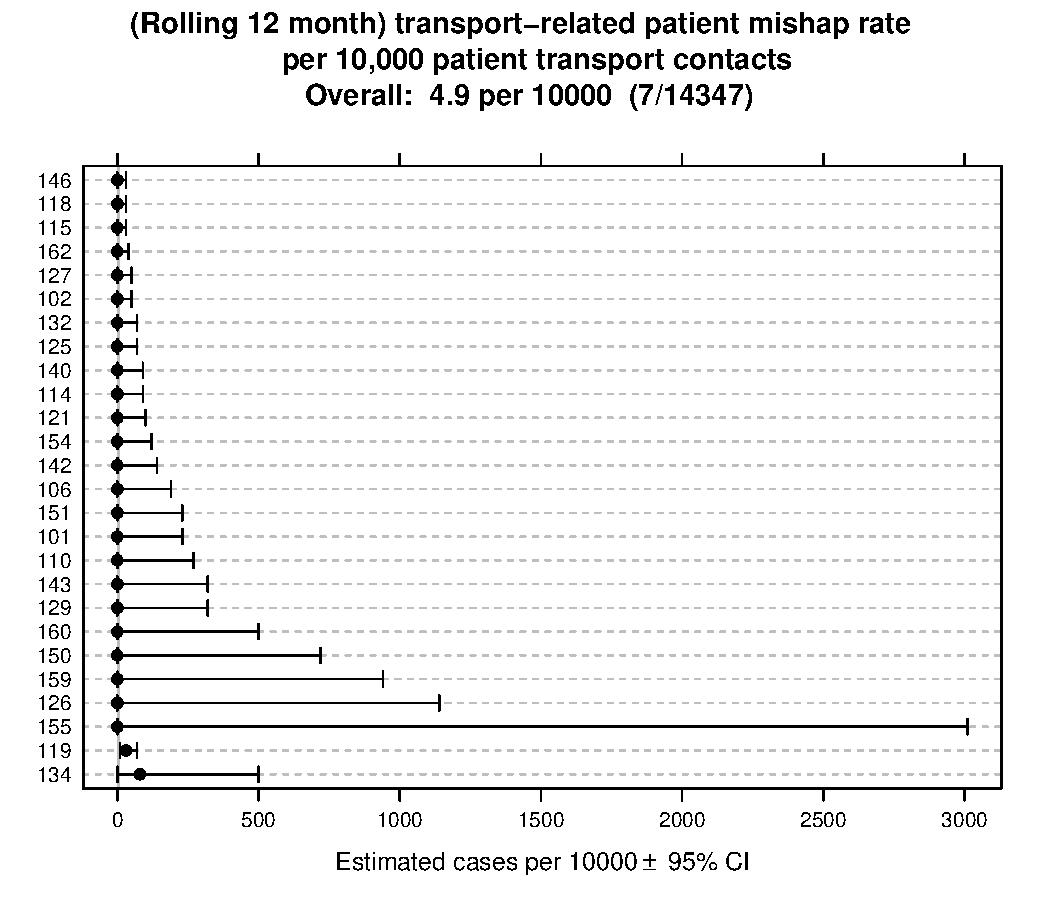
\includegraphics{figures/nearmiss.pdf}

\end{frame}

\begin{frame}{Rate of Serious Reportable Event}

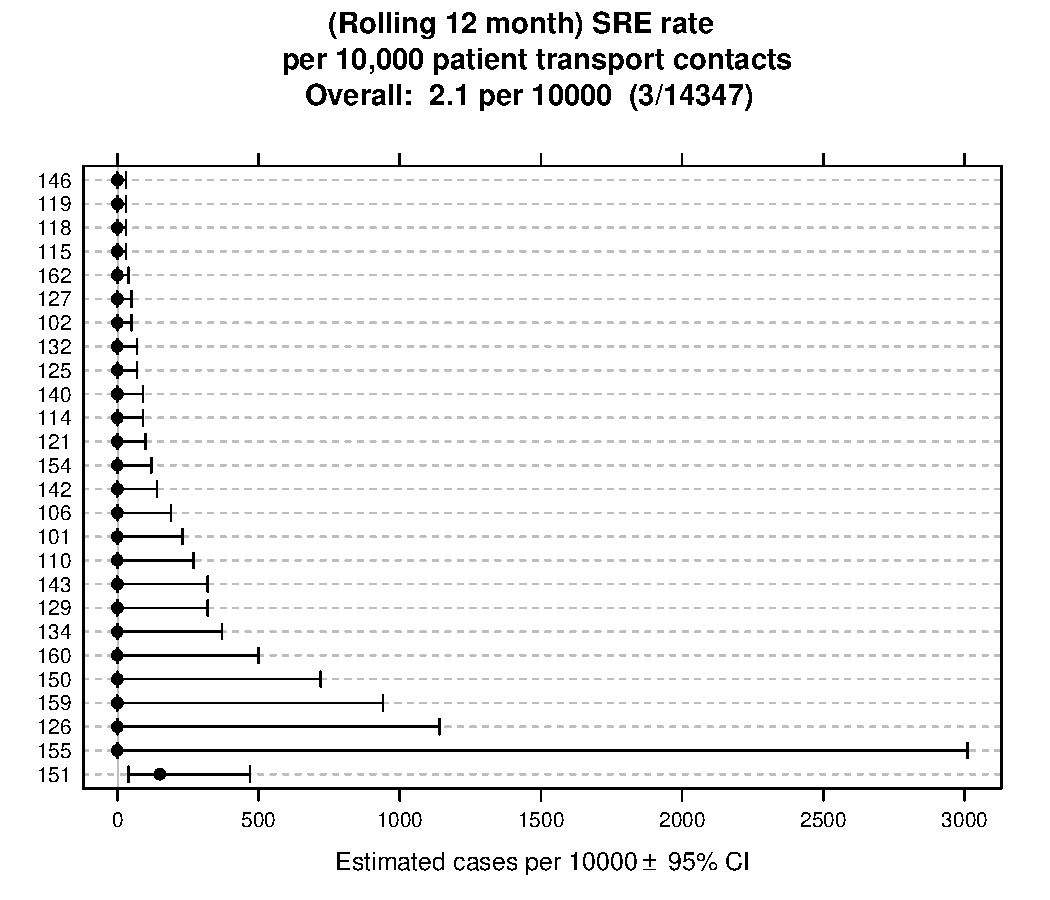
\includegraphics{figures/sre.pdf}

\end{frame}

\begin{frame}{Unplanned device dislodgements}

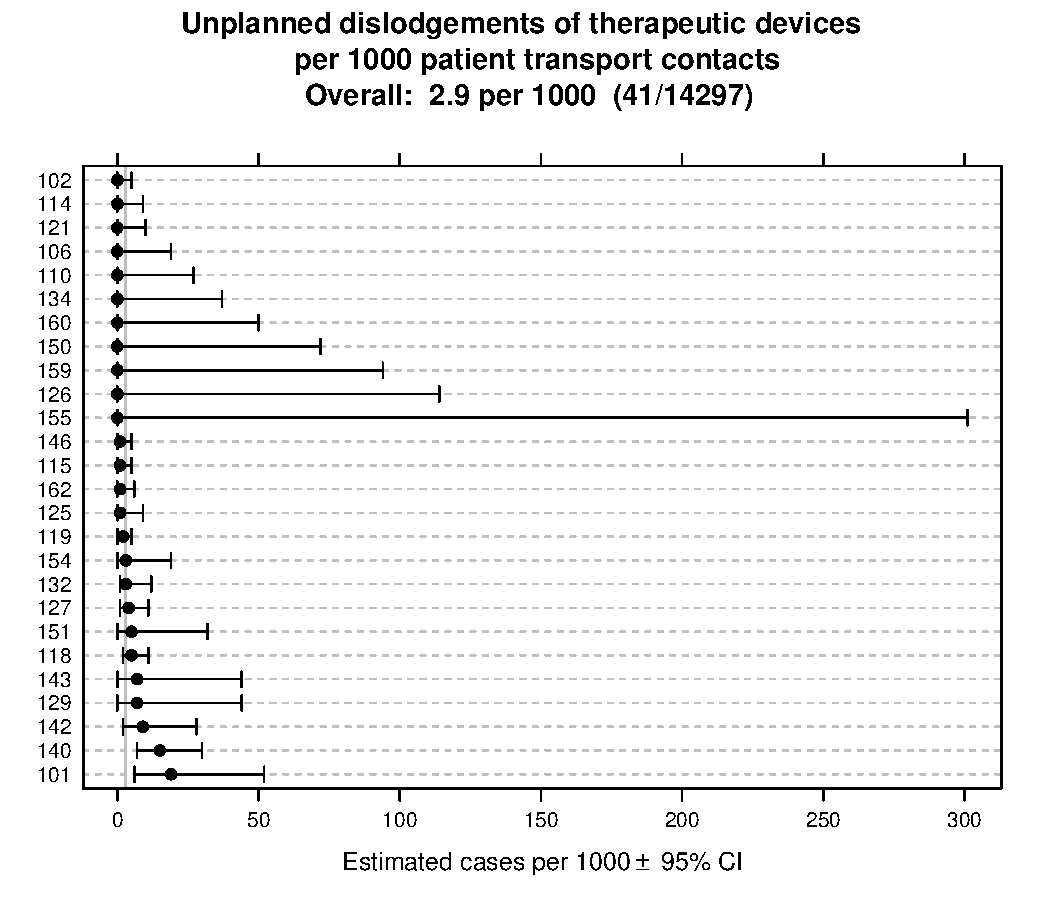
\includegraphics{figures/device_dislogement.pdf}

\end{frame}

\begin{frame}{Medication errors on transport}

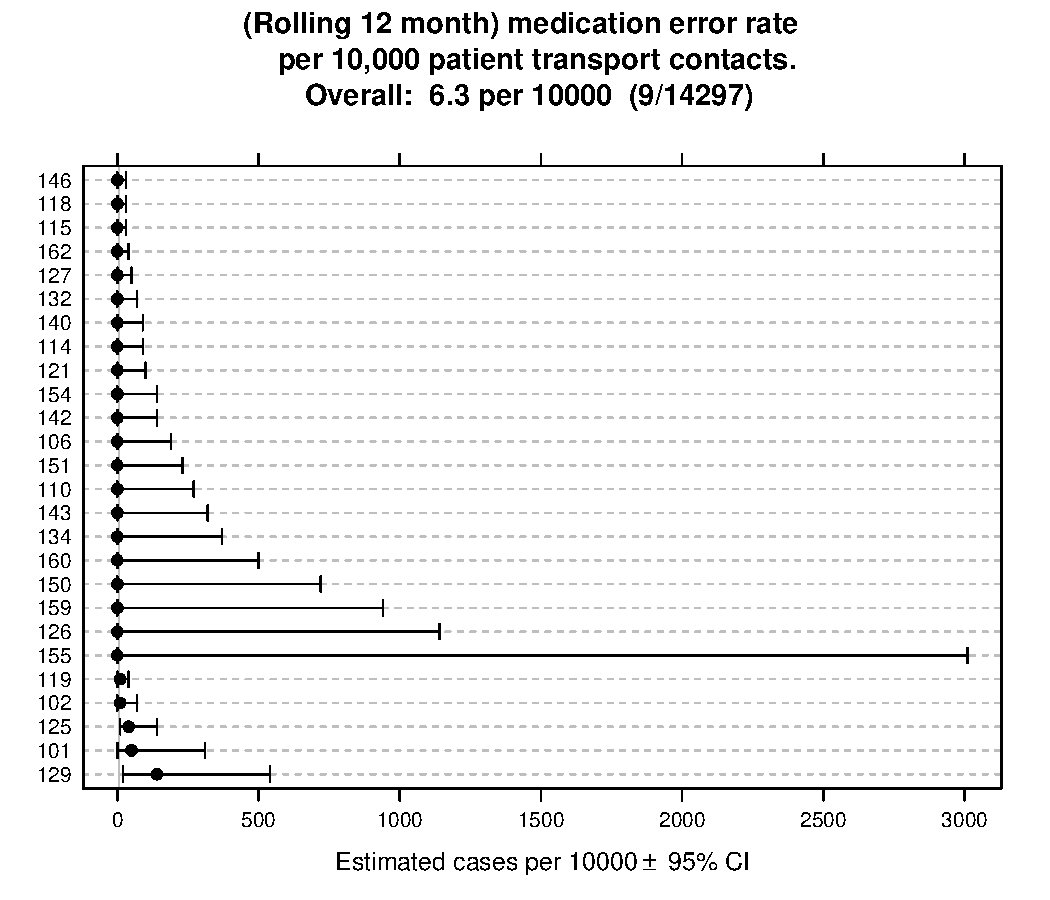
\includegraphics{figures/med_error.pdf}

\end{frame}

\end{document}
